\documentclass[11pt,a4j,uplatex]{jsarticle}
\usepackage{ascmac}
\usepackage{amsmath}
\usepackage[dvipdfmx]{graphicx}
\usepackage{upgreek}
\usepackage{ulem}
\usepackage{bm}%ベクトル表記\bm{なにか}
\usepackage{cases}%連立方程式

\newsavebox{\circlebox}
\savebox{\circlebox}{\fontencoding{OMS}\selectfont\Large\char13}
\newlength{\circleboxwdht}
\newcommand{\centercircle}[1]{%
  \setlength{\circleboxwdht}{\wd\circlebox}%
  \addtolength{\circleboxwdht}{\dp\circlebox}%
  \raisebox{0.4\dp\circlebox}{%
    \parbox[][\circleboxwdht][c]{\wd\circlebox}{\centering#1}}%
  \llap{\usebox{\circlebox}}%
}	%丸数字(文字)環境。\centercircle{入れたい文字} で丸文字を表示する。


\title{宮島研究室2019年度B4 XRD実験}
\author{東京理科大学 理学部 応用物理学科\\宮島研究室B4 渡辺慧}
\date{\today}


\begin{document}

\maketitle %タイトル

\thispagestyle{empty}%このページにはページ番号を入れない.
\clearpage
\addtocounter{page}{-1}%ページのカウントを-1する.

\newpage

\tableofcontents %目次

\thispagestyle{empty}%このページにはページ番号を入れない
\clearpage
\addtocounter{page}{-1}

%\listoffigures%図目次。確認用。後で消す

\newpage
\section{本研究の目的}
なんとか

\newpage
\section{原理}

\subsection{結晶面}

図\ref{a1}(a)のような立方格子を考える。$\bm{a_1}、\bm{a_2}、\bm{a_3}$を各方向への単位ベクトルと考えた時、位置ベクトル$\bm{r}$は$\bm{r}=h\bm{a_1}+k\bm{a_2}+l\bm{a_3}$と表せる。$h,k,l$はミラー指数と呼ばれる。このとき、$\bm{r}$の方向を[$h,k,l$]と表記する。[$h,k,l$]方向のベクトルと直交する面を格子面と呼ぶ。格子面は、図\ref{a1}(b)のように等間隔に無限に並び、その間隔を$d_{hkl}$とする。原点から$d_{hkl}$の距離にある面を($h,k,l$)と表記する。また、($h,k,l$)と平行な面すべてを内包して\{$h,k,l$\}と表記する。($h,k,l$)は、各方向の単位長さを1としたとき、それぞれの軸の$\frac{1}{h}$、$\frac{1}{k}$、$\frac{1}{l}$の位置を通過する。ただし、方向成分が0の方向があるとき、格子面はその方向と平行になる。
%その間隔$d_{hkl}$は$\frac{hkl}{n!\sqrt{h^2+k^2+l^2}}$である(ただし、値が0であるの指数があるとき、その文字を取り除いて考える。また、$n$は、0でない指数の数である)。
\begin{figure}[ht]
 \centering
 \begin{tabular}{c}

  \begin{minipage}{0.5\hsize}
   \centering
   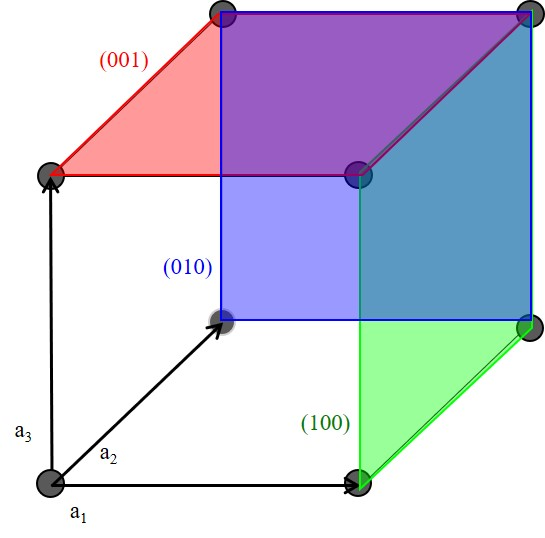
\includegraphics[clip, width=4.5cm]{a1.jpg}
   \hspace{2cm} (a)
  \end{minipage}

  \begin{minipage}{0.5\hsize}
   \centering
   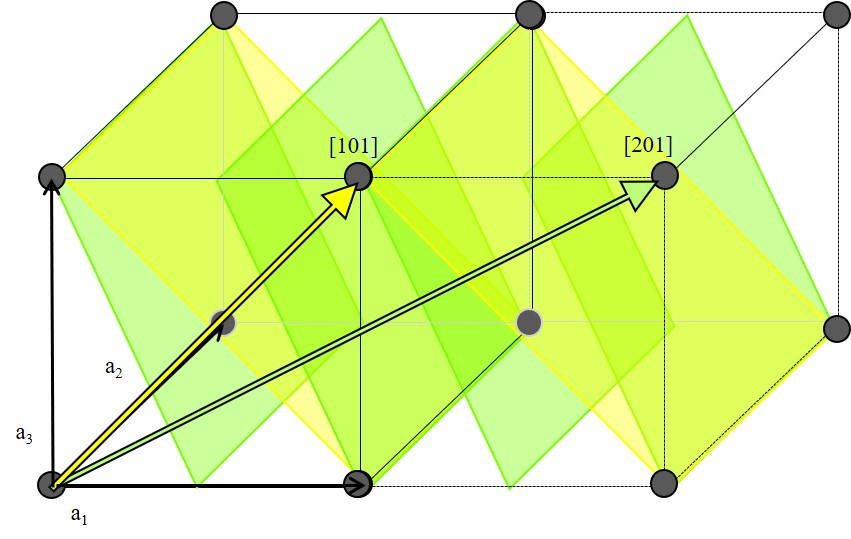
\includegraphics[clip, width=6cm]{a2.jpg}
   \hspace{2cm} (b)
  \end{minipage}

 \end{tabular}
 \caption{結晶面の概形.}
 \label{a1}

\end{figure}

\newpage
\subsection{逆格子}
結晶の構造においては、単位格子が空間的に繰り返す周期性がある。ここで、並進操作$\bm{r}\to\bm{r+R}$に対し不変となるベクトル
\begin{equation}
\bm{R}=n_a\bm{a_1}+n_b\bm{a_2}+n_c\bm{a_3}
\nonumber
\end{equation}
が存在する。$\bm{R}$を実格子ベクトルと呼ぶ。ここで、結晶と同様の周期性を持つ関数$\phi(\bm{r})=\phi(\bm{r+R})$を波数ベクトル$\bm{G}$でフーリエ展開すると、
\begin{equation}
  \phi(\bm{r})=\sum_{\bm{G}}\phi_{\bm{G}}e^{i\bm{G\cdot r}}
  \label{r}
\end{equation}

\begin{equation}
  \phi(\bm{r+R})=\sum_{\bm{G}}\phi_{\bm{G}}e^{i\bm{G\cdot (r+R)}}
  \label{r+R}
\end{equation}

となる。ここで、式(\ref{r})と式(\ref{r+R})は等しいため、$\bm{R}$と$\bm{G}$は
\begin{equation}
e^{i\bm{G\cdot R}}=1\leftrightarrow\bm{G\cdot R}=2n\pi
  \label{GR}
\end{equation}
を満たさなければならない。このような$\bm{G}$を
\begin{equation}
\bm{G}=h\bm{b_1}+k\bm{b_2}+l\bm{b_3}
\nonumber
\end{equation}
と定義する。$hkl$は回折指数である。$\bm{G}$を逆格子ベクトルと呼び、$(長さ)^-1$の次元を持つ。この時、$\bm{a}_j$と$\bm{b}_k$の間には、
\begin{equation}
\bm{a}_j\cdot\bm{b}_k=\delta_{jk}
\end{equation}
\begin{numcases}
{}
\delta_{jk}=0(j\neq k)\\
\delta_{jk}=2\pi(j=k)
\nonumber
\end{numcases}
の関係がある。ここで、$|a_1|=|a_2|=|a_3|$かつ$|b_1|=|b_2|=|b_3|$のとき、$|b_j|=\frac{1}{|a_j|}$である。
$l=0$のときの、実格子空間と逆格子空間の簡単な対応を図\ref{kousi}に示す。
\begin{figure}[htb]
 \centering
 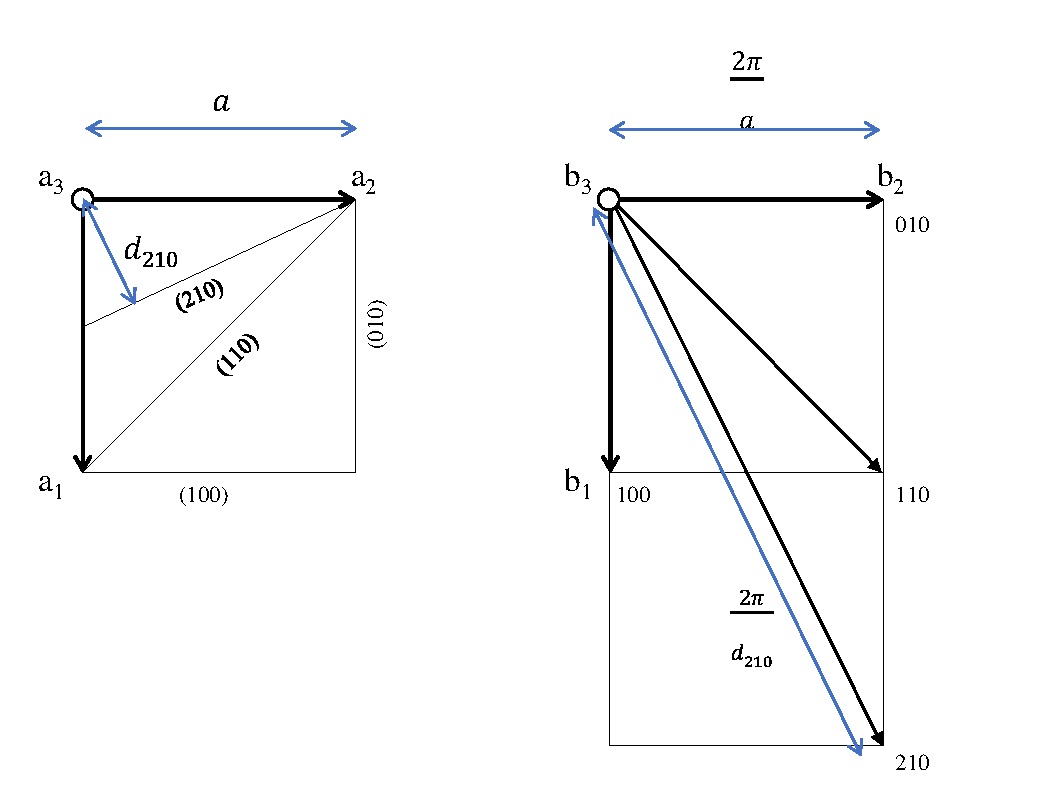
\includegraphics[clip,width=10cm]{kousi.eps}
 \caption{実格子と逆格子の関係.}
 \label{kousi}
\end{figure}

\newpage
左が実格子空間、右が逆格子空間である。$hkl=210$を見てみると、逆格子ベクトル[210]は、実格子における(210)と垂直である。また、$\bm{G}_{hkl}$方向の結晶面の間隔$d_{hkl}$は
\begin{equation}
  d_{hkl}=\frac{2\pi}{|\bm{G}_{hkl}|}\times \mathrm{gcd}(h,k,l)
\end{equation}
と表せる。gcd$(h,k,l)$は$(h,k,l)$の最大公約数である。最大公約数が1であるとき、つまり$(h,k,l)$の組が互いに素であるとき、回折指数$hkl$とミラー指数$(h,k,l)$は一致する。



\newpage
\subsection{回折条件}
実格子空間でのX線の回折の条件を考える。X線がある結晶面によって散乱を起こすときの光路を図\ref{dsinq}に示す。入射光と結晶面の角度を$\theta$、結晶面の間隔を$d$としたとき、この時、2つの光の光路差は$2d\sin\theta$である。散乱前後で光の波長が変化しないとき、この光路差がX線の波長の整数倍であれば、散乱光は強め合う。よって、実格子空間におけるX線の回折の条件は
\begin{equation}
 2d\sin\theta=n\lambda
 \label{bragg}
\end{equation}
となる。この条件をBragg条件と呼ぶ。

\begin{figure}[htb]
 \centering
 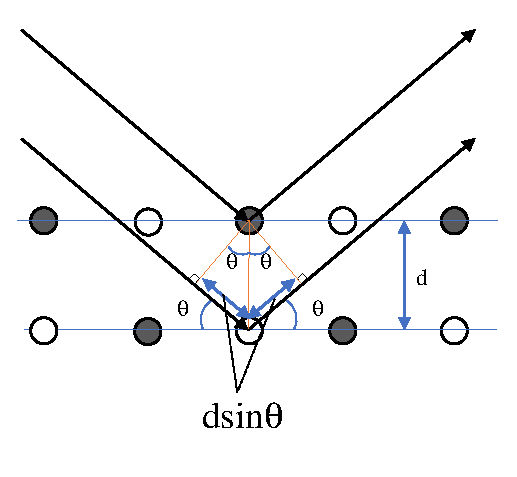
\includegraphics[clip,width=5cm]{dsinq.eps}
 \caption{実格子空間におけるX線の散乱.}
 \label{dsinq}
\end{figure}

また、逆格子空間でのX線の回折の条件を考える。入射X線の波数ベクトルを$\bm{k_0}$、散乱X線の波数ベクトルを$\bm{k}$とする。逆格子空間におけるX線の散乱を図\ref{hasuu}に示す。
$\bm{k_0}$が逆格子空間の原点を向くベクトルだと考えると、$\bm{k}$の終着点は$\bm{k_0-k}$で表せる(これを散乱ベクトルと呼ぶ)。ここで、散乱ベクトルが逆格子ベクトル$\bm{G}_{hkl}$と等しいとき、つまり、散乱X線の波数ベクトルの終点が逆格子空間の格子点に等しいとき、回折が起きる。したがって、逆格子空間におけるX線の回折の条件は、
\begin{equation}
 \bm{k-k_0}=\bm{G}_{hkl}
 \label{laue}
\end{equation}
となる。この条件をLaue条件と呼ぶ。

\begin{figure}[htb]
 \centering
 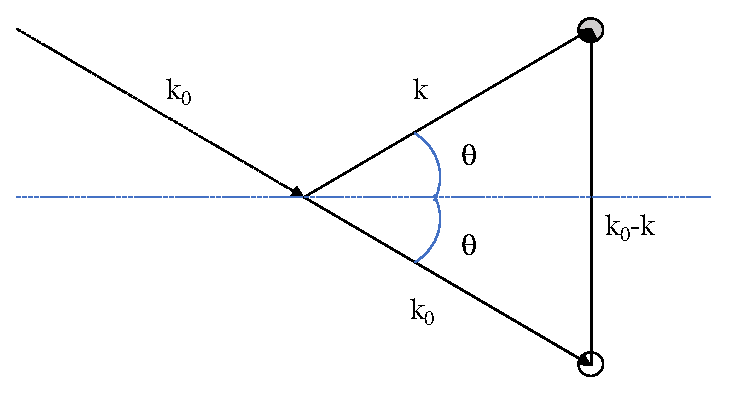
\includegraphics[clip,width=6cm]{hasuu.eps}
 \caption{逆格子空間におけるX線の散乱.}
 \label{hasuu}
\end{figure}

\if0
\newpage%ここいる?
図\ref{hasuu}を見ると、入射X線と散乱X線のなす角が$2\theta$であることがわかる。ここで、Thomson散乱を考えるとき、散乱前後で波数は変化しないので、$\bm{|k_0|=|k|}$である。よって、
\begin{equation}
 \bm{2|k|}\sin\theta=|\bm{G}_{hkl}|
 \nonumber
\end{equation}
である。これに、$\bm{|k|}=\frac{2\pi}{\lambda}$と、$|\bm{G}_{hkl}|=\frac{2\pi}{d_{hkl}}$を代入すると、
\begin{equation}
 2\cdot\frac{2\pi}{\lambda}\sin\theta=\frac{2\pi}{d_{hkl}}
 \nonumber
\end{equation}
が導ける。これを変形するとBraggの条件と一致するので、式(\ref{bragg})と式(\ref{laue})は等価である。
\fi

\newpage
\subsection{X線回折}%ここいる?
X線は電磁波であり、結晶にX線を入射したとき、X線は構成原子の原子核と電子によって散乱される。荷電粒子による電磁波の散乱には、散乱波の波長が元の波長から変化しないThomson散乱と、散乱はの波長が元の波長よりも長くなるCompton散乱の2種類がある。Thomson散乱は干渉性散乱、Compton散乱は非干渉性散乱である。結晶による回折においては、干渉性散乱のみを考えればよいので、Thomson散乱のみを考える。Thomson散乱において、散乱断面積は散乱体の質量の自乗に反比例するため、X線は電子により散乱される。
密度$\rho(\bm{r})$で空間分布した電子雲によってX線が散乱される場合を、図\ref{sanran}を用いて考える。
\begin{figure}[htb]
 \centering
 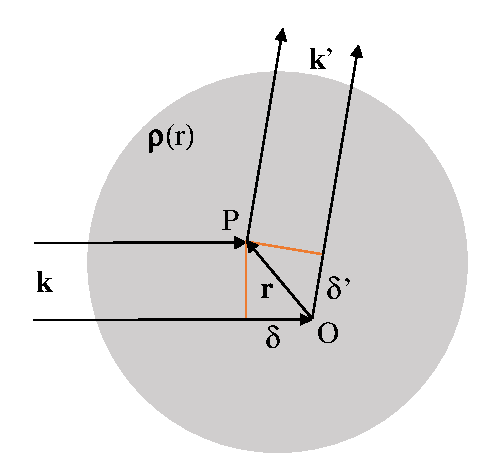
\includegraphics[clip,width=5cm]{sanran.eps}
 \caption{電子雲によるX線の散乱.}
 \label{sanran}
\end{figure}

電子雲に平面波のX線が入射して、原点Oと点Pで波数$\bm{k}$から$\bm{k}'$に散乱された時、位相差は
\begin{equation}
  \delta_1+\delta_2=\bm{(-k\cdot r)+(k'\cdot r)}=K\cdot r
\end{equation}
と表せる(散乱ベクトル$\bm{K=k'-k}$を定義した)。
この時、ある散乱先$\bm{r'}$における散乱X線の重ね合わせは
\begin{equation}
  A\rho\bm{(0)}e^{i(\bm{k'\cdot r'})}+  A\rho\bm{(r)}e^{i(\bm{k'\cdot r'+\delta_1+\delta_2})}=A[\rho\bm{(0)}e^{i(\bm{K\cdot 0})}+\rho\bm{(r)}e^{i(\bm{K\cdot r})}]e^{i(\bm{k'\cdot r'})}
\end{equation}
となる(A:定数)。ここで、右辺の[]内の項は、点O、Pで散乱されたX線の振幅に等しい。よって、電子雲全体での散乱振幅は、
\begin{equation}
  f=\int\rho(\bm{r})e^{i\bm{K\cdot r}}d\bm{r}
  \label{insi}
\end{equation}
に比例することがわかる。

\newpage
ところで、$\rho(\bm{r})$は、結晶の構成原子それぞれの電子密度の和
\begin{equation}
  \rho(\bm{r})=\sum_{\bm{R}}\sum_j\rho_j(\bm{r-[R+}\bm{r}_j])
\end{equation}
で表せる($\bm{r}_j$:結晶中のj番目の原子の位置ベクトル)。これを用いて式(\ref{insi})を変形すると、
\begin{equation}
  \begin{split}
  f&=\int\rho(\bm{r})=\sum_{\bm{R}}\sum_j\rho_j(\bm{r-R-}\bm{r}_j)e^{i\bm{K\cdot r}}d\bm{r}\\
  &=\sum_{\bm{R}}e^{i\bm{K\cdot R}}\sum_je^{i\bm{K}\cdot\bm{r}_j}\int\rho_j(\bm{r-R-}\bm{r}_j)e^{i\bm{K\cdot (\bm{r-R-}\bm{r}_j)}}d\bm(r)\\
  &=\sum_{\bm{R}}e^{i\bm{K\cdot R}}\sum_jf_je^{i\bm{K}\cdot\bm{r}_j}
\end{split}
\end{equation}
となる。式(\ref{insi})より、$\int\rho_j(\bm{r-R-}\bm{r}_j)e^{i\bm{K\cdot (\bm{r-R-}\bm{r}_j)}}=f_j$とした。結晶全体の散乱の和を$\sum_{\bm{R}}e^{i\bm{K\cdot R}}\equiv G(\bm{K})$、単位格子中の散乱の和を$\sum_jf_je^{i\bm{K}\cdot\bm{r}_j}\equiv F(\bm{K})$と定義する。
$G(\bm{K})$はLaue関数と呼ばれ、Laueの回折条件を満たすとき有限の値をとり、それ以外の場合はほぼ0である。一例として、あああああああ(教科書写す)
$G(\bm{K})$がLaue関数であることから、$F(\bm{K})$について、$\bm{K}=\bm{G}_{hkl}$として計算できる。よって、
\begin{equation}
\begin{split}
    F_{hkl}&=\sum_jf_je^{i\bm{G}_{hkl}\cdot\bm{r}_j}\\
    &=\sum_jf_je^{2\pi i(h\bm{b_1}+k\bm{b_2}+l\bm{b_3})}
\end{split}
\end{equation}
となる。$F_{hkl}$を結晶構造因子と呼ぶ。結晶構造因子はLaue関数と同様、特定の条件を満たすとき有限の値をとり、それ以外の場合は0である。したがって、Laue条件を満たしていても、$F_{hkl}=0$のとき回折は観測されない。これを消滅則と呼ぶ。格子の形状によって、有限の値をとる条件が異なるため、結晶構造の解析の際に有用である。

\newpage
\subsection{NaClの結晶構造}
NaCl結晶は。、NaCl型構造をとる。NaClの構造の概形を図\ref{nacl}に示す。

\begin{figure}[htb]
 \centering
 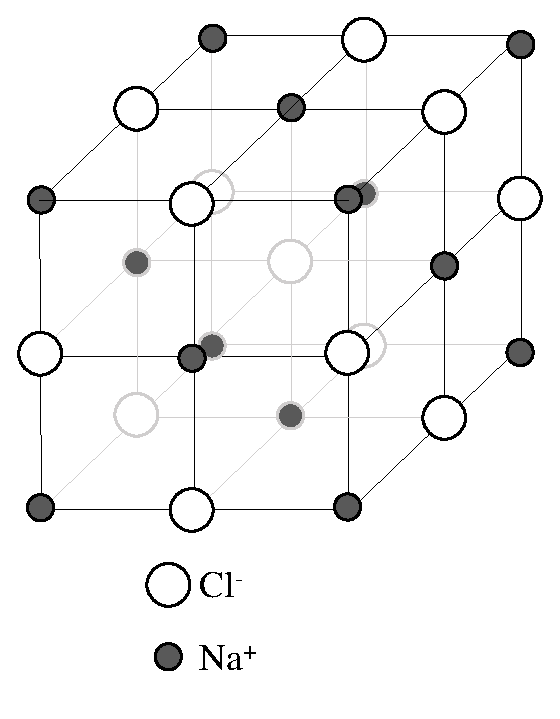
\includegraphics[clip,width=8cm]{nacl.eps}
 \caption{NaClの結晶構造.}
 \label{nacl}
\end{figure}

すこし消滅則の話

\newpage
\subsection{$2\theta/\theta$法}

単結晶の時は(002)、粉末の場合はいろんな面がーーってのを書く。

\newpage
\subsection{NaCl粉末の回折パターン}

$2\theta$の値が90よりも小さいときの、NaCl粉末の回折パターンを表\ref{data}に示す。実験データの解析のおいては、この表のデータを参照する。

\begin{table}[htbp]
 \begin{center}
  \caption{NaCl粉末の回折パターン\cite{powder}.}
  \begin{tabular}{|r|r|r|r|r|r|}  \hline
                           & \multicolumn{3}{c|}{} &   &                                \\
   $2\theta(\mathrm{deg})$ & h                     & k & l & Intensity & d-spacing [nm] \\  \hline \hline
   26.886                  & 1                     & 1 & 1 & 10        & 0.3312         \\
   31.145                  & 2                     & 0 & 0 & 99        & 0.2869         \\
   44.629                  & 2                     & 2 & 0 & 61        & 0.2028         \\
   52.878                  & 3                     & 1 & 1 & 3         & 0.173          \\
   55.426                  & 2                     & 2 & 2 & 19        & 0.1656         \\
   64.959                  & 4                     & 0 & 0 & 8         & 0.1434         \\
   71.633                  & 3                     & 3 & 1 & 2         & 0.1316         \\
   73.797                  & 4                     & 2 & 0 & 19        & 0.1283         \\
   82.251                  & 4                     & 2 & 2 & 13        & 0.1171         \\
   88.472                  & 5                     & 1 & 1 & 2         & 0.1104         \\ \hline
  \end{tabular}
  \label{data}
 \end{center}
\end{table}

\newpage
\section{NaCl粉末及び単結晶の回折パターンの観測方法}

NaCl粉末及び単結晶の回折パターンを、X線回折装置"SmartLab"を用いて観測した。$\mathrm{SmartLab}$の構造を図\ref{smartlab}に示す。

\begin{figure}[htb]
 \centering
 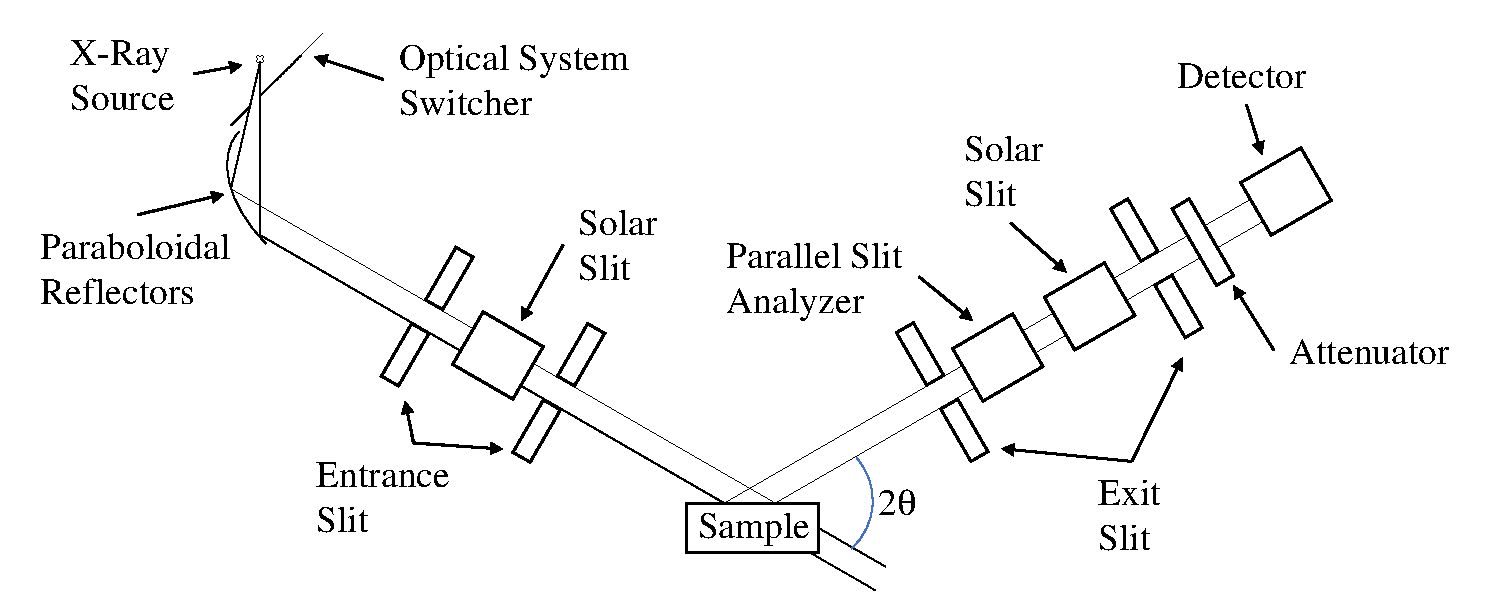
\includegraphics[clip,width=12cm]{XRD.eps}
 \caption{SmartLabの内部構造.}
 \label{smartlab}
\end{figure}

X線源から放射された光をNaCl粉末及び単結晶に照射し、光検出器で回折光を観測した。X線源から等方的に放射された光を、放物面人工多層膜ミラーを用いて単色化・平行化し、2枚の入射スリットとソーラースリットを用いて発散を制限した。2枚の出射スリットとソーラースリットを用いて、試料からの回折光の発散を制限した。アッテネーターを用いて、光検出器に入射する光を減衰させた。PSA(平行スリットアナライザー)を用いて分解能を決定した。$2\theta$は入射光と出射光のなす角である。表\ref{exp}の実験条件の下、試料ごとに$2\theta$を変えてゆき、回折パターンを測定した。試料はNaCl粉末とNaCl単結晶の2種類である。単結晶試料の寸法を図\ref{size}に示す。

\begin{table}[ht]
 \centering
 \caption{実験条件.}
 \begin{tabular}{lc}\hline
  \multicolumn{2}{c}{実験条件}          \\ \hline
  入射スリット     & 1 mm               \\
  出射スリット     & 1 mm               \\
  ソーラースリット & 0.5 deg            \\
  X線波長          & 1.543\AA、1.392\AA \\\hline
 \end{tabular}
 \label{exp}
\end{table}

\begin{figure}[htb]
 \centering
 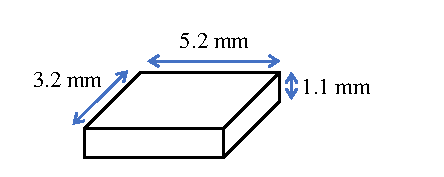
\includegraphics[clip,width=9cm]{bulk.eps}
 \caption{NaCl単結晶の寸法.}
 \label{size}
\end{figure}


\newpage
実験に用いた単結晶は、縦3.2 mm、横5.2 mm、高さ1.1 mmの直方体のものである。この結晶を、最も面積の広い面を下にして試料台に設置した。

\newpage
\section{NaCl粉末及び単結晶の回折パターンの解析}


\subsection{NaCl粉末}

NaCl粉末における回折パターンを図\ref{powder}に示す。

\begin{figure}[htb]
 \centering
 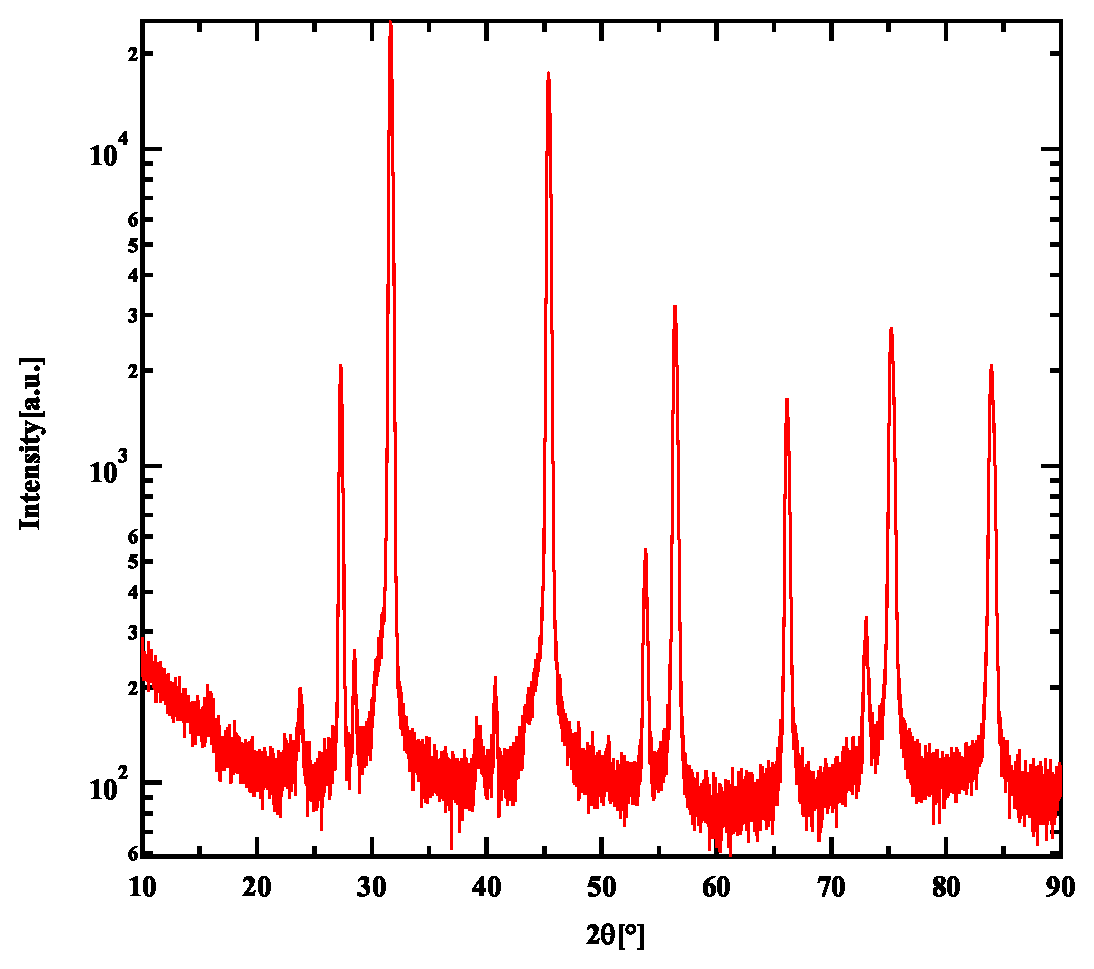
\includegraphics[clip,width=7cm]{FigPowder.eps}
 \caption{NaCl粉末の回折パターン.}
 \label{powder}
\end{figure}

横軸は入射光と回折光のなす角、縦軸は回折強度である。グラフから、鋭いピークが複数見られる。これらのピークのうち、頂点における$2\theta$が、表\ref{data}の値と近いものだけを抜き出したものを表\ref{pow}に示す。

\begin{table}[htbp]
 \begin{center}
  \caption{NaCl粉末の格子定数.}
  \begin{tabular}{|c|r|c|lll|c|}  \hline
   $2\theta[\mathrm{deg}]$ & \multicolumn{1}{c|}{$2\theta[\mathrm{rad}]$} & $G_{m}$     & h & k & l & a           \\ \hline  \hline
   27.306                  & 0.468753                                     & 1.891361571 & 1 & 1 & 1 & 5.751031023 \\
   31.646                  & 0.543256333                                  & 2.185068392 & 2 & 0 & 0 & 5.748103832 \\
   45.397                  & 0.779315167                                  & 3.093719005 & 2 & 2 & 0 & 5.741478885 \\
   53.828                  & 0.924047333                                  & 3.63032518  & 3 & 1 & 1 & 5.737338297 \\
   56.419                  & 0.968526167                                  & 3.791544409 & 2 & 2 & 2 & 5.737650888 \\
   66.178                  & 1.136055667                                  & 4.381295096 & 4 & 0 & 0 & 5.733464524 \\
   73.041                  & 1.2538705                                    & 4.777872498 & 3 & 3 & 1 & 5.729304283 \\
   75.259                  & 1.291946167                                  & 4.902560146 & 4 & 2 & 0 & 5.728642375 \\
   83.979                  & 1.4416395                                    & 5.375122452 & 4 & 2 & 2 & 5.723700519 \\  \hline
  \end{tabular}
  \label{pow}
 \end{center}
\end{table}

\newpage
逆格子ベクトルの大きさ$G_{m}$は
\begin{equation}
 G_m=\frac{4\pi}{\uplambda}\sin\theta
 \label{gyakukousi}
\end{equation}
で計算した。$\uplambda$は、今回は$K_\alpha$線の波長である1.543 nmを用いた。格子定数$a$は、$G_{m}$から
\begin{equation}
 a=\frac{2\pi}{G_m}\sqrt{h^2+k^2+l^2}
 \label{kousiteisuu}
\end{equation}
で計算した。各$\theta$におけるaの平均をとって、格子定数は
\begin{equation}
 \nonumber
 a=5.736746
 \label{complete}
\end{equation}
と求まった。

\newpage
\subsection{NaCl単結晶}



図\ref{bulk}に示す。

\begin{figure}[htb]
 \centering
 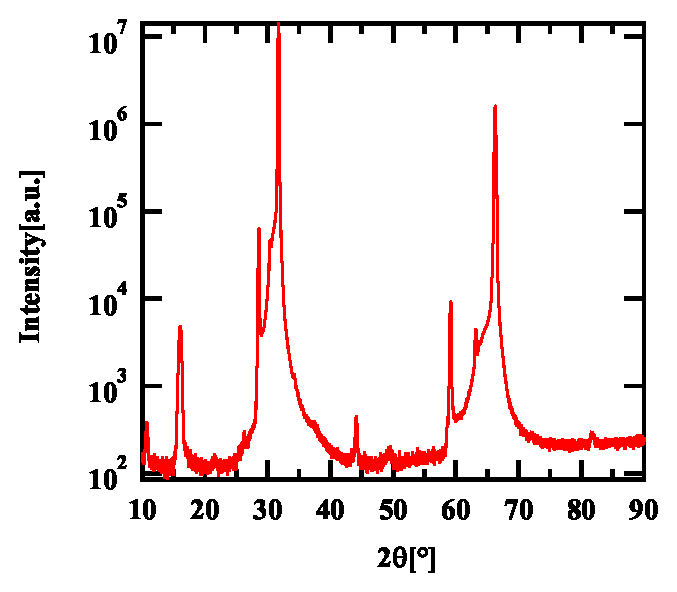
\includegraphics[clip,width=9cm]{FigBulk.eps}
 \caption{NaCl単結晶の回折パターン.}
 \label{bulk}
\end{figure}

横軸はAの回転角、縦軸は回折強度である。グラフから、鋭いピークが複数見られる。$2\theta/\theta$法を用いた単結晶のX線回折測定では、(001)面に平行な面での回折しか観測できないため、$K_\alpha$線及び$K_\beta$線の二つのX線による回折が観測できる。したがって、どのピークが、どのX線による回折を示しているのか判断ができない。$2\theta/\theta$法を用いた単結晶のX線回折測定では、(001)面に平行な面での回折しか観測できないことを利用し、(h,k,l)=(0,0,2n)となるように回折指数をとり、粉末試料で得た格子定数に近い計算結果が得られるよう、$2\theta$を逆算した。その結果を表\ref{gyakusan}に示す。

\begin{table}[htbp]
 \begin{center}
  \caption{2$\theta$の見積もり.}
  \begin{tabular}{|c|c|c|c|c|}\hline
   $a$        & $\lambda$ & l & $\theta$[rad] & 2$\theta$[deg] \\  \hline  \hline
   5.73674607 & 1.39      & 2 & 0.244733355   & 28.04437672    \\
   5.73674607 & 1.54      & 2 & 0.271778272   & 31.14349589    \\
   5.73674607 & 1.39      & 4 & 0.505900419   & 57.97191777    \\
   5.73674607 & 1.54      & 4 & 0.566746084   & 64.94431732    \\ \hline
  \end{tabular}
  \label{gyakusan}
 \end{center}
\end{table}

\newpage
表\ref{gyakusan}から、$K_\alpha$線及び$K_\beta$線由来の、(0,0,2n)面による回折角が見積もれた。図\ref{bulk}のピークのうち、頂点における2$\theta$が、表\ref{gyakusan}に近いものだけを抜き出したものを表\ref{crystal}に示す。

\begin{table}[htbp]
 \begin{center}
  \caption{NaCl単結晶の格子定数.}
  \begin{tabular}{|c|c|c|c|ccc|c|c|c|}  \hline
   $2\theta[\mathrm{deg}]$ & $2\theta[\mathrm{rad}]$ & $G_{m\beta}$       & $G_{m\alpha}$      & h & k & l & $a_\beta$          & $a_\alpha$         \\   \hline  \hline
   28.598                  & 0.490932333             & 2.195818211        & \sout{1.982945083} & 0 & 0 & 2 & 5.71996349         & \sout{6.334013034} \\
   31.739                  & 0.544852833             & \sout{2.431301177} & 2.195599203        & 0 & 0 & 2 & \sout{5.165958095} & 5.72053405         \\
   59.173                  & 1.015803167             & 4.394597543        & \sout{3.968564221} & 0 & 0 & 4 & 5.716109326        & \sout{6.329745117} \\
   66.28                   & 1.137806667             & \sout{4.867753959} & 4.395850588        & 0 & 0 & 4 & \sout{5.160490899} & 5.714479939        \\  \hline
  \end{tabular}
  \label{crystal}
 \end{center}
\end{table}

%単結晶においては、(001)面に平行な面での回折のみが見られることから、$K_\beta$線による回折も観測できる。そのため、各回折指数hklにおいて、2つの格子定数が計算できる。この逆算から、特性X線$K_\alpha$と$K_\beta$による1次と2次の回折角が得られた。それを図\ref{kakb}に示す。
逆格子ベクトルの大きさ$G_m$および格子定数$a$は、NaCl粉末と同様の方法で計算した。$\lambda$は表\ref{gyakusan}のように、$K_\alpha$線による回折は1.543 nm、$K_\beta$線による回折は1.392 nm をもちいた。各$\theta$における$a$の平均をとって、格子定数は
\begin{equation}
 \nonumber
 a=5.717771701
 \label{complete2}
\end{equation}
と求まった。
\if0
 \begin{figure}[htb]
  \centering
  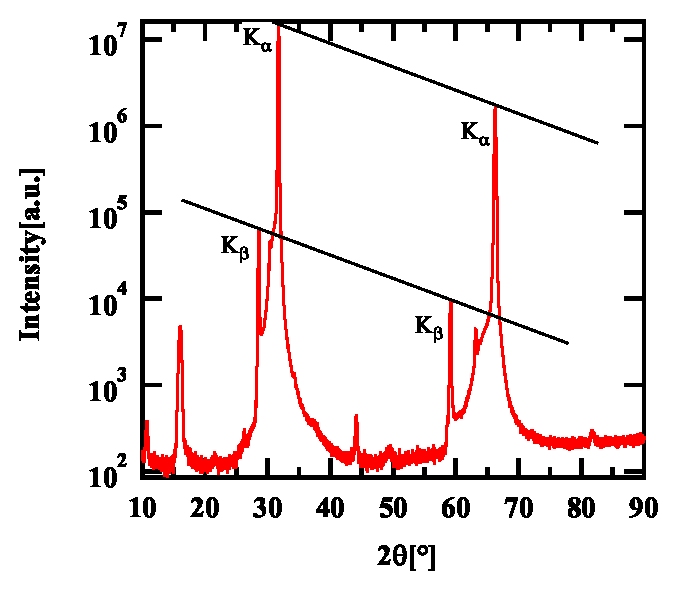
\includegraphics[clip,width=9cm]{kakb.eps}
  \caption{NaCl結晶の回折パターン.}
  \label{kakb}
 \end{figure}
\fi

\newpage

\if0%ここいらない
 ブラッグの回折条件より、$2d\sin\theta=n\lambda$である。よって、表\ref{kakb}の値から、[001]方向の面間隔を計算できる。計算結果を表\ref{d}に示す。%ここいる?

 \begin{table}[htbp]
  \begin{center}
   \caption{NaCl単結晶の面間隔.}
   \begin{tabular}{|l|l|}  \hline
    2[deg] & d           \\  \hline  \hline
    28.598 & 2.859981745 \\
    31.739 & 2.861717794 \\
    59.173 & 2.858054663 \\
    66.28  & 2.858689203 \\ \hline
   \end{tabular}
   \label{d}
  \end{center}
 \end{table}

 各$\theta$における$d$の平均をとって、面間隔は
 \begin{equation}
  d=2.859610851
  \label{fin}
 \end{equation}
 と求まった。
\fi

\section{結論}
かんとか

\newpage
%参考文献。\cite{タグ}で参照を示せる。
\begin{thebibliography}{9}
 \bibitem{powder}株式会社島津 https://www.shimadzu.co.jp/products/opt/guide/07.html 2019/4/12
 \bibitem{CCD} キヤノンサイエンスラボ https://global.canon/ja/technology/s\_labo/light/003/04.html 2019/04/12
 \bibitem{Fibor} 分光計器株式会社 http://www.bunkoukeiki.co.jp/technology.fiber.html 2019/04/12
 \bibitem{varshni}Y.P.Varshni TEMPERATURE DEPENDENCE OF THE ENERGY GAP IN SEMICONDUCTORS
 \bibitem{gapE}キッテル固体物理学入門上第8版 p.119


\end{thebibliography}

\end{document}
